%!TEX root = main.tex
\section{Use Case: Smart Room Control}

\begin{frame}
\frametitle{Use Case}

The described algorithms are combined into an \textbf{IOT} application implementing a \textbf{NUI} system that is integrated into the \textbf{SYNAISTHISI} platform.

This system is used to \textbf{control the devices} inside in the \textbf{Aigaio} meeting room which is located in IIT Demokritos.

\end{frame}

% %!TEX root = main.tex
\subsection{The Internet of Things}


\begin{frame}
\frametitle{IoT definition}
The Internet of Things is <insert preferred definition>.
\end{frame}


\begin{frame}
\frametitle{IoT definition}
The Internet of Things is a generalization of the World Wide Web to incorporate ``things'' that exist in the physical world. 
\end{frame}

\begin{frame}
\frametitle{IoT definition}
The Internet of Things is the convergence of all virtual and physical entities that are able to produce, consume and act upon data under a common communications infrastructure.
\end{frame}

\begin{frame}
\frametitle{Synaisthisi Platform}
The Synaisthisi platform is a project developed in NCSR Demokritos that aims to facilitate the development of Internet of Things applications.

It provides
\begin{itemize}
\item A \textbf{Service Oriented Architecture} where applications can be developed as the composition of small functional building blocks (services) 
\item A categorization of services in Sensing, Processing and Actuating (\textbf{SPA services})
\item A \textbf{Message Oriented Middleware} that provides a pub/sub message passing infrastructure based on MQTT for inter-service communication
\item Mechanisms for logging, security, persistent storage, data replication and administration of the applications and the system
\end{itemize}
\end{frame}


\begin{frame}
\frametitle{Synaisthisi Architecture}

\begin{figure}[!htb]
\centering
\resizebox{0.85\linewidth}{!}{
	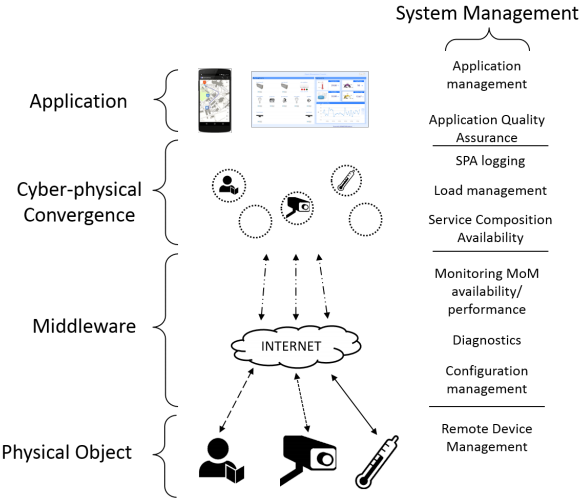
\includegraphics[]{figs/synaisthisi-arch}
}
\end{figure}

\end{frame}

% %!TEX root = main.tex
\subsection{Machine to Machine Communication}


\begin{frame}
\frametitle{Publish/Subscribe Protocols}
Pros:

\begin{itemize}
\item \textbf{Asynchronous} communication
\item \textbf{Decoupling} of the communicating entities
\item \textbf{Many to many} communication
\item \textbf{Scalable}
\end{itemize}

Cons:
\begin{itemize}
\item \textbf{Semantic coupling} (message type needs to be statically defined)
\item \textbf{Loose} message delivery \textbf{guarantees}
\end{itemize}

\end{frame}


\begin{frame}
\frametitle{MQTT}

All of the above plus
\begin{itemize}
\item Lightweight
\item Small code footprint
\item Small header overhead
\item QoS Levels
\end{itemize}

\begin{figure}[!htb]
\centering
\resizebox{0.85\linewidth}{!}{
	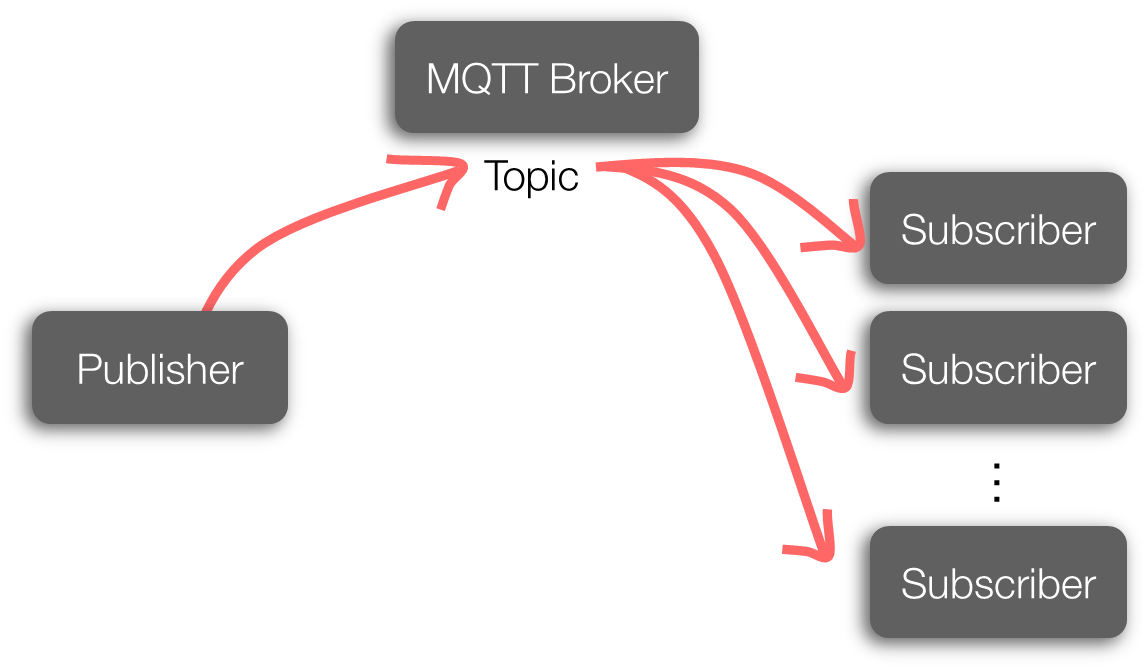
\includegraphics[]{figs/mqtt-block-diagram}
}
\end{figure}

\end{frame}


\subsection{System Design}

\begin{frame}
\frametitle{Aigaio Devices}
\Wider[1em] {
\begin{figure}
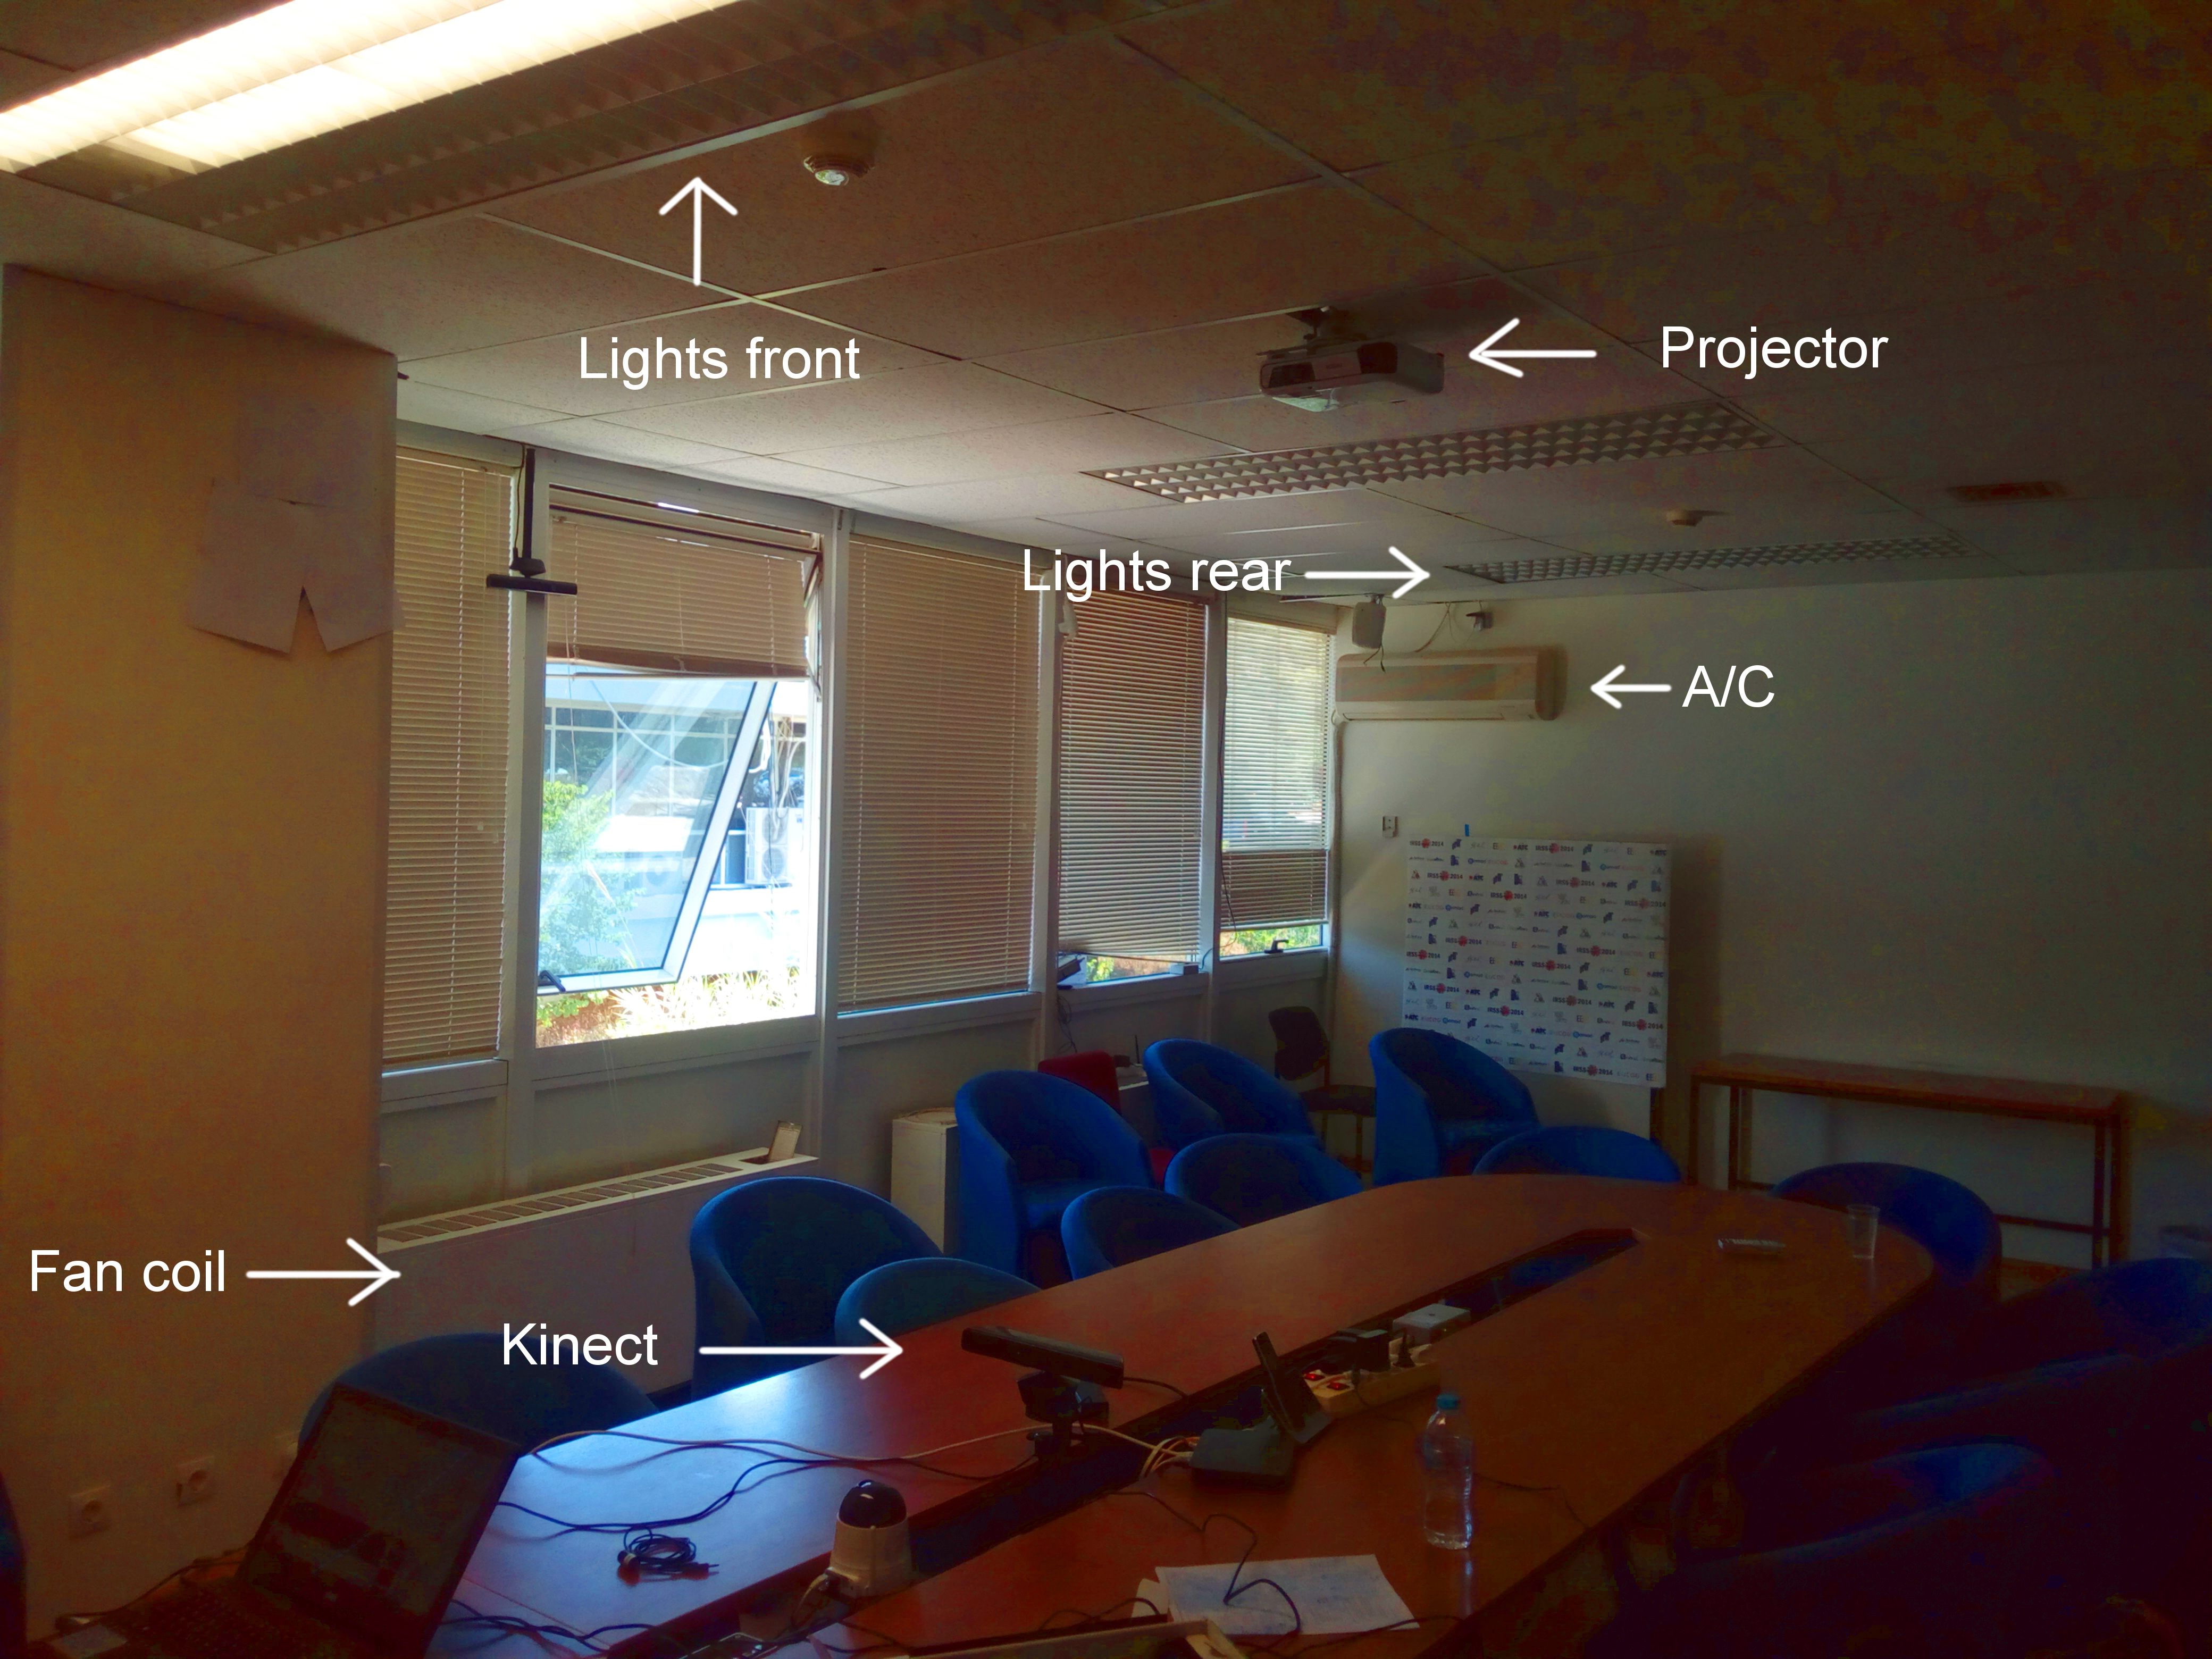
\includegraphics[width=\columnwidth]{figs/aigaio}
\end{figure}
}
\end{frame}

\begin{frame}
\frametitle{Aigaio Devices}

\begin{table}
\centering
\resizebox{0.7\columnwidth}{!}{
\begin{tabular}{l l | l l}
        /pw2                & Projector & /pw3     & Lights Front \\
        /pw4                & A/C       & /pw5     & Fan Coils \\
        /pw6                & Fan Coils & /pw8     & Lights Rear \\
        /ir\_control/action & IR Module &
    \end{tabular}
}
\end{table}

\begin{figure}[ht!]
\centering
\resizebox{\columnwidth}{!}{

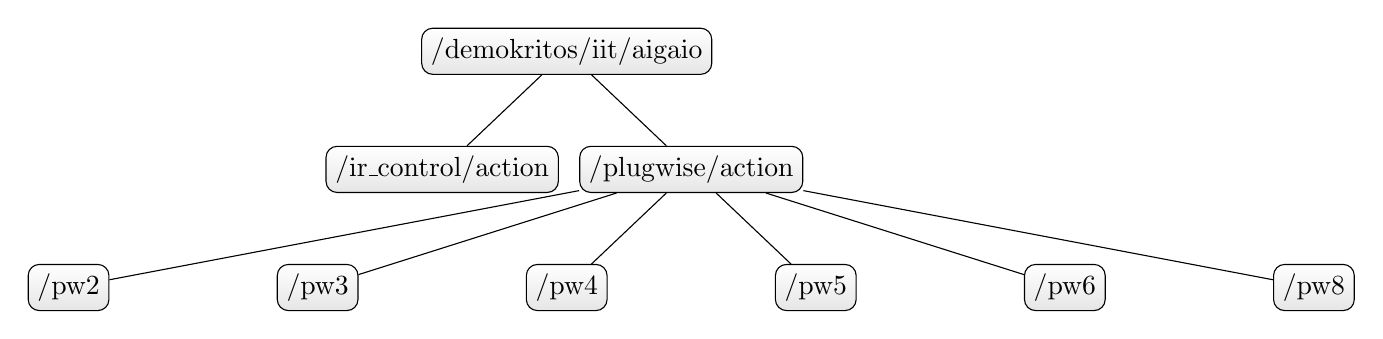
\begin{tikzpicture}[sibling distance=9em,
  every node/.style = {shape=rectangle, rounded corners,
    draw, align=center,
    top color=white, bottom color=gray!20}]]
  \node {/demokritos/iit/aigaio} 
    child { node {/ir\_control/action} }
    child { node {/plugwise/action}
    	child { node {/pw2} }
    	child { node {/pw3} }
    	child { node {/pw4} }
    	child { node {/pw5} }
    	child { node {/pw6} }
    	child { node {/pw8} }
  };
\end{tikzpicture}
}
\end{figure}

\end{frame}


\begin{frame}
\frametitle{Aigaio NUI components}
\Wider[5em]{

\begin{figure}[!htb]
\centering
\resizebox{\columnwidth}{!}{
	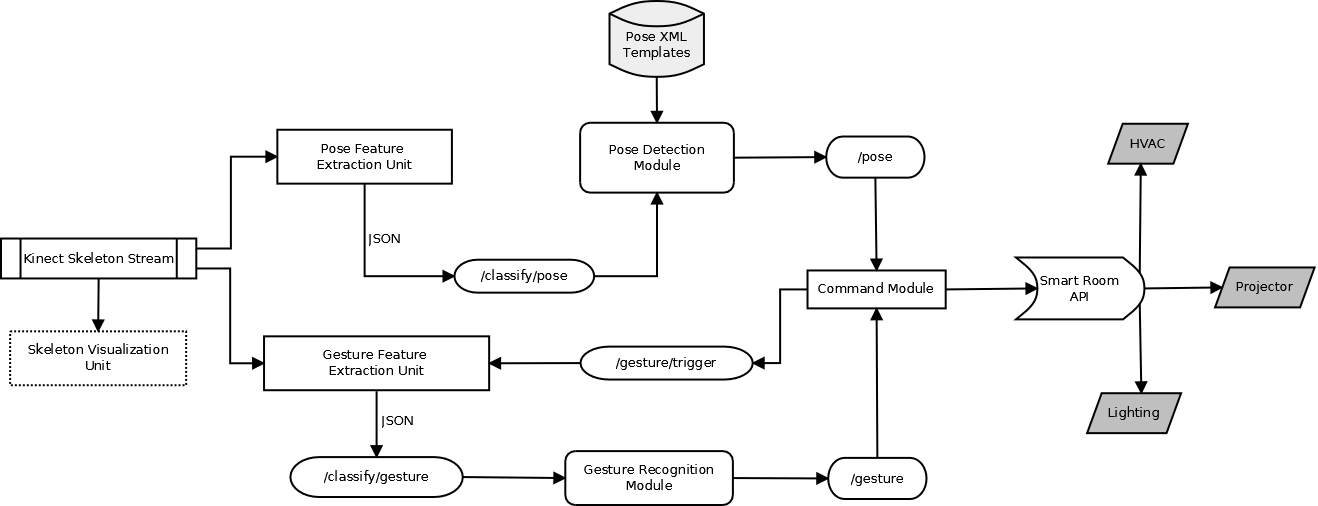
\includegraphics[]{figs/block-diagram}
}
\end{figure}
}

\end{frame}


\begin{frame}
\frametitle{Aigaio NUI services}
\Wider[5em]{

\begin{figure}[!htb]
\centering
\resizebox{\columnwidth}{!}{
	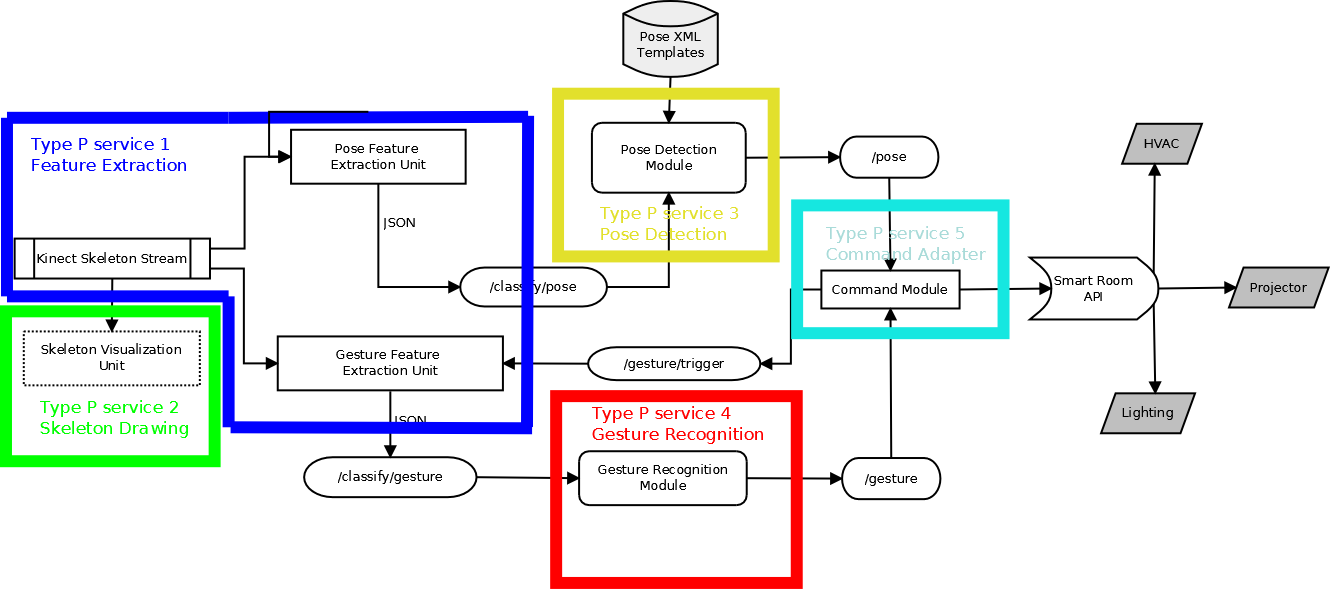
\includegraphics[]{figs/block-diagram-services}
}
\end{figure}
}

\end{frame}


\begin{frame}
\frametitle{Aigaio NUI technology stack}
\Wider[5em]{

\begin{figure}[!htb]
\centering
\resizebox{\columnwidth}{!}{
	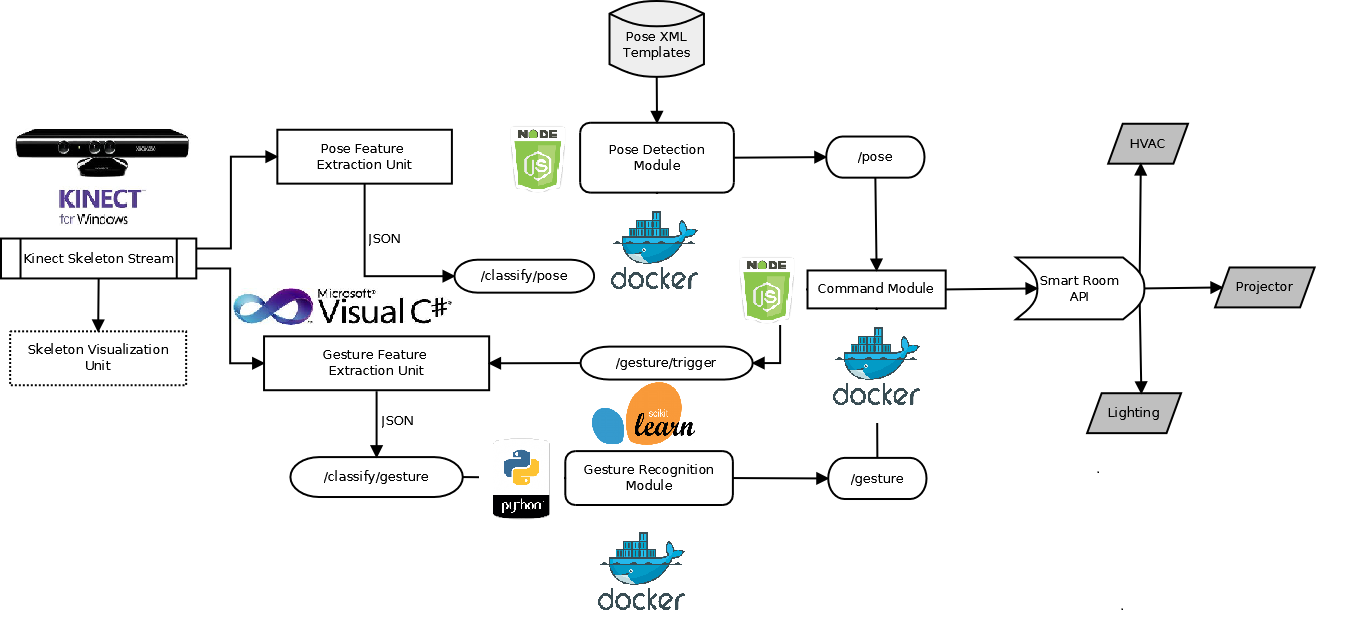
\includegraphics[]{figs/block-diagram-tech}
}
\end{figure}
}
\end{frame}

